% vim: ai sw=2 spell spelllang=cs

\iffimuni
\section{Chyby souběhu}
\fi

\begin{frame}[fragile]
  \frametitle{Chyby souběhu, zámky}

  \heading{LDD3 kap. 5} (zastaralá)

  \bigskip

  \heading{Co je chyba souběhu}
  \begin{itemize}
  \item Chyba závislá na načasování/prokládání operací
  \end{itemize}

  \medskip

  \begin{block}{Ukázkový kód}
  \begin{lstlisting}[language=C]
int *addr = &some_int;
...
int a = load(addr);
a = a + 1;
store(a, addr);
  \end{lstlisting}
  \end{block}

\end{frame}

\begin{frame}[fragile]
  \frametitle{Příklad chyby souběhu}

  \begin{center}
  \begin{tabular}{c}
  \begin{lstlisting}[language=C]
int a = load(addr);
a = a + 1;
store(a, addr);
  \end{lstlisting}
  \end{tabular}

  \smallskip

  Uvažujme při startu \code{*addr == 0}

  \bigskip
  \pause

  \begin{tabular}{c|c|c}
  \code{*addr} & Vlákno A & Vlákno B \\ \hline
  \begin{lstlisting}[language=C]
0
0
0
  \end{lstlisting} &
  \begin{lstlisting}[language=C]
int a = load(addr);
a = a + 1;
<schedule>
  \end{lstlisting} &
  \begin{lstlisting}[showlines]
<waiting>         ~


  \end{lstlisting} \\
  \end{tabular}
  \end{center}

  \pause

  \begin{center}
  \begin{tabular}{c|c|c}
  \code{*addr} & Vlákno A & Vlákno B \\ \hline
  \begin{lstlisting}[language=C]
0
0
1
  \end{lstlisting} &
  \begin{lstlisting}[language=C]
int a = load(addr);
a = a + 1;
<waiting>
  \end{lstlisting} &
  \begin{lstlisting}[language=C]
int a = load(addr);
a = a + 1;
store(a, addr);
  \end{lstlisting}
  \end{tabular}
  \end{center}

  \pause

  \begin{center}
  \begin{tabular}{c|c|c}
  \code{*addr} & Vlákno A & Vlákno B \\ \hline
  \begin{lstlisting}[language=C]
   0
   0
/*>1<*/
  \end{lstlisting} &
  \begin{lstlisting}[language=C]
int a = load(addr);
a = a + 1;
store(a, addr);
  \end{lstlisting} &
  \begin{lstlisting}[language=C,showlines]
<exited>          ~


  \end{lstlisting}
  \end{tabular}
  \end{center}
\end{frame}

\begin{frame}
  \frametitle{Řešení chyb souběhu}

  \begin{itemize}
  \item Atomickou operací ve stylu \code{load_inc_store}
  \begin{itemize}
  \item Nutná podpora CPU
  \item Ne na všechno jsou operace (vesměs jen +, -, load, store)
  \end{itemize}

  \pause

  \item Kritickou sekcí
  \begin{itemize}
  \item Kus kódu vykonávaný max.\ jedním procesem
  \item Zámky
  \end{itemize}

  \pause

  \item Read-copy-update (RCU)
  \begin{itemize}
  \item Podrobnosti v LDD
  \end{itemize}
  \end{itemize}
\end{frame}

\mysection{Atomické operace, bitmapy}

\begin{frame}[fragile]
  \frametitle{Atomické operace}

  \begin{itemize}
  \item \header{linux/atomic.h}, \doc{Documentation/atomic\_ops.txt}
  \item \code{atomic_t a = ATOMIC_INIT(5)}
  \item Pojme 32 bitů se znaménkem (\code{int}) (historicky jen 24)
  \item \code{atomic_read}, \code{atomic_set}
  \item \code{atomic_add}, \code{atomic_inc}, \code{atomic_sub},
    \code{atomic_dec}, \code{atomic_*_return} a další (LXR)
  \end{itemize}

  \pause

  \begin{block}{Řešení pomocí atomických operací}
  \begin{center}
  \begin{tabular}{ccc}
  \begin{lstlisting}[language=C]
int *addr = &some_int;
...
int a = load(addr);
a = a + 1;
store(a, addr);
  \end{lstlisting} & $\Rightarrow$ &
  \begin{lstlisting}[language=C]
atomic_t a;
...
atomic_inc(&a);
/* nebo atomic_add(1, &a); */
  \end{lstlisting}
  \end{tabular}
  \end{center}
  \end{block}

  \pause

  \begin{itemize}
  \item \code{atomic64_t} (drahý na 32-bitu)
  \end{itemize}

\end{frame}

\begin{frame}
  \frametitle{Úkol}

  \heading{Práce s atomickými typy}
  \begin{enumerate}
    \item Definujte jeden \code{atomic_t} v \code{module_init}
    \item Nastavte hodnotu na -3 (nejlépe staticky)
    \item Atomicky \emph{jednou} operací proveďte ,,přičíst 1 a přečíst
      hodnotu''
    \item Přečtenou hodnotu vypište do logu
    \item Přičtěte 3
    \item Odečtěte 1
    \item Přičtěte hodnotu a vraťte jako návratovou z \code{module_init}
  \end{enumerate}

  \bigskip

  Pozn.: tento kód nemažte, budeme s ním nadále pracovat
\end{frame}

\begin{frame}
  \frametitle{Atomické bitové operace}

  \begin{itemize}
  \item Stačí-li 1 bit namísto celého čísla (např.\ \code{int})
  \item \header{linux/bitops.h}, \doc{Documentation/atomic\_ops.txt}
  \item \code{DECLARE_BITMAP(a, 1000)}
  \item \code{set_bit}, \code{clear_bit}, \code{test_bit}
  \item \code{test_and_set_bit}, \code{test_and_clear_bit}
  \end{itemize}

  \pause
  \medskip

  \heading{Bitmapy lze použít i NEATOMICKY (např.\ v kritických sekcích)}
  \begin{itemize}
  \item \header{linux/bitmap.h}
  \item \code{__set_bit}, \code{__clear_bit}
  \item \code{bitmap_zero}, \code{bitmap_fill}, \code{bitmap_copy}
  \item \code{bitmap_OP}, kde $\text{\code{OP}} \in \left\{\text{\code{and}},
    \text{\code{or}}, \text{\code{xor}}, \text{\code{andnot}},
    \text{\code{complement}}\right\}$
  \item \code{bitmap_empty}, \code{bitmap_full}, \dots
  \end{itemize}

\end{frame}

\begin{frame}
  \frametitle{Úkol}

  \heading{Práce s bitmapami}
  \begin{enumerate}
    \item Definujte bitové pole o 100 bitech
    \item Vymažte obsah pole
    \begin{itemize}
      \item \code{bitmap_zero}
    \end{itemize}

    \item Nastavte 2., 63.\ a 76.\ bitu (čísla považujte za indexy v C)
    \item Vypište \emph{long} (\code{\%lx}) s 63.\ bitem
    \begin{itemize}
      \item \code{bitmapa[BIT_WORD(63)]}
    \end{itemize}

    \item Vypište celou bitmapu jako řetězec
    \begin{itemize}
      \item \code{bitmap_scnprintf} (do 4.0), \code{\%*bp} (od 4.0)
    \end{itemize}

    \item Vypište \emph{longy} obsahující bity nastavené na 1
    \begin{itemize}
      \item \code{for_each_set_bit}
    \end{itemize}

    \item Vypište \emph{pozici} 1.\ nastaveného bitu
    \begin{itemize}
      \item \code{find_first_bit}
    \end{itemize}
  \end{enumerate}
\end{frame}

\mysection{Zámky}

\begin{frame}
  \frametitle{Zámky}

  \heading{Vytvoření kritické sekce}
  \begin{itemize}
    \item Spinlocky
    \begin{itemize}
      \item Čekání ve smyčce (požírá strojový čas)
      \item Rychlé, ale \pozor: nesmí se uvnitř spát (čekat)
    \end{itemize}

    \pause

    \item Mutexy
    \begin{itemize}
      \item Spící, fronta čekatelů
      \item Pomalejší než spinlock (viz tělo \code{__mutex_lock_common})
    \end{itemize}

    \pause

    \item Semafory
    \begin{itemize}
      \item Podobné mutexům
      \item Počítadlo (jsou rekurzivní)
      \item Dnes se používají výjimečně
    \end{itemize}
  \end{itemize}

  \medskip
  \pause

  \begin{center}
  \heading{\pozor \\ Zámky lze držet jen v jádře (po dobu vykonávání
  syscallu)}
  \end{center}
\end{frame}

\iffimuni
\subsection{Spinlocky}
\fi

\begin{frame}[fragile]
  \frametitle{Zámky v jádře -- spinlocky}

  \begin{itemize}
    \item Čekání ve smyčce
    \item \header{linux/spinlock.h}, \doc{Documentation/spinlocks.txt}
    \item \code{DEFINE_SPINLOCK(lock)}, \code{spinlock_t lock}
    \item \code{spin_lock}, \code{spin_unlock}
    \item Podobné \code{pthread} spinlockům
  \end{itemize}

  \pause

  \begin{block}{Řešení pomocí spinlocků}
  \begin{center}
  \begin{tabular}{ccc}
  \begin{lstlisting}[language=C]
int *addr = &some_int;
...
int a = load(addr);
a = a + 1;
store(a, addr);
  \end{lstlisting} & $\Rightarrow$ &
  \begin{lstlisting}[language=C]
DEFINE_SPINLOCK(addr_lock);
int *addr = &some_int;
...
spin_lock(&addr_lock);
int a = load(addr);
a = a + 1;
store(a, addr);
spin_unlock(&addr_lock);
  \end{lstlisting}
  \end{tabular}
  \end{center}
  \end{block}

\end{frame}

\begin{frame}
  \frametitle{Úkol}

  \heading{Práce se spinlocky}
  \begin{enumerate}
  \item Úkol s atomickými operacemi přepište
  \item \code{atomic_t} změnte na obyčejný \code{int} 
  \item A celý kód obalte spinlockem
  \item Vyzkoušejte
  \end{enumerate}

\end{frame}

\iffimuni
\subsection{Mutexy}
\fi

\begin{frame}[fragile]
  \frametitle{Zámky v jádře -- mutexy}

  \heading{Mutexy}
  \begin{itemize}
    \item Spící, fronta čekatelů
    \item \header{linux/mutex.h}
    \item \code{DEFINE_MUTEX(name)}
    \item \code{mutex_lock}, \code{mutex_unlock}
    \item Podobné \code{pthread} mutexům
  \end{itemize}

  \pause

  \begin{block}{Řešení pomocí mutexů}
  \begin{center}
  \begin{tabular}{ccc}
  \begin{lstlisting}[language=C]
int *addr = &some_int;
...
int a = load(addr);
a = a + 1;
store(a, addr);
  \end{lstlisting} & $\Rightarrow$ &
  \begin{lstlisting}[language=C]
DEFINE_MUTEX(addr_lock);
int *addr = &some_int;
...
mutex_lock(&addr_lock);
int a = load(addr);
a = a + 1;
store(a, addr);
mutex_unlock(&addr_lock);
  \end{lstlisting}
  \end{tabular}
  \end{center}
  \end{block}

\end{frame}

\begin{frame}
  \frametitle{Zámky v jádře -- ostatní}

  \heading{Semafory}
  \begin{itemize}
  \item \header{linux/semaphore.h}
  \item Víceméně nepoužívat
  \item Pozor: \code{DECLARE\_MUTEX(lock)}
  \item \code{down}, \code{up}
  \end{itemize}

  \pause
  \medskip
  \medskip

  \heading{Big Kernel Lock (BKL)}
  \begin{itemize}
    \item Historický
    \begin{itemize}
      \item Dnes už v jádře nenajdeme (commit 4ba8216cd9 v 2.6.39)
      \item Jen jeho relikty
    \end{itemize}
    \item Hrubozrnný
    \item Pochází z dob počátku Linuxu
    \item \code{lock_kernel}, \code{unlock_kernel}
  \end{itemize}

\end{frame}

\begin{frame}{Úkol}

  \heading{Atomické čtení/zápis bufferu o velikosti 128 bytů} \iffimuni
    (součást domácího) \fi
  \begin{enumerate}
    \item Globální buffer 128 B

    \item 2 znaková (misc) zařízení
    \begin{itemize}
      \item 1 implementuje \code{.read}
      \item 1 implementuje \code{.write}
    \end{itemize}

    \item Zápis
    \begin{itemize}
      \item Umožněn max.\ po 5 znacích (\code{.write} vrací max.\ 5)
      \item Spí 20~ms po každém zápisu \emph{znaku} do bufferu (\code{get_user}
        a \code{msleep} z \header{linux/delay.h})
    \end{itemize}

    \item Čtení
    \begin{itemize}
      \item Vrátí naráz celých 128 B (je-li \code{count} dostatečně velký)
      \item Musí vidět změny pouze po 5 znacích (až na poslední kousek)
    \end{itemize}

    \item Vyzkoušejte
  \end{enumerate}

  \medskip

  Pozn.: inspirace v pb173/04\\

\end{frame}

\begin{frame}[fragile]
  \frametitle{Deadlock}

  \begin{itemize}
    \item 4 podmínky uváznutí
    \item Jádro spoléhá na programátora, že k němu nikdy nedojde
    \item \textsc{LockDep}
    \begin{itemize}
      \item Dynamický mechanismus hledání chyb v zámcích
    \end{itemize}
    \item Obvyklé typy chyb: ABBA, AA
    \item Obvyklé chyby: \code{lock} + \code{if} + \code{return} (\pozor)
  \end{itemize}

  \begin{figure}
  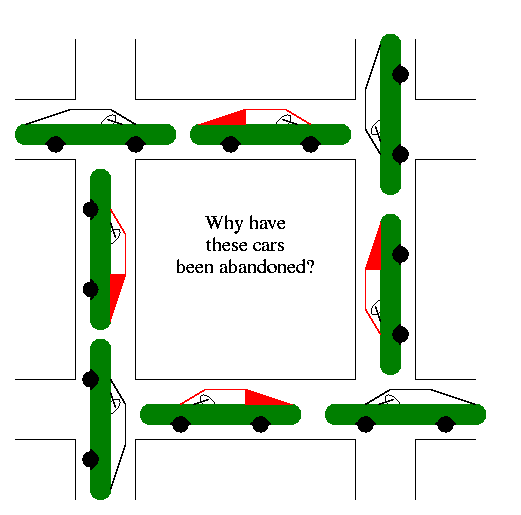
\includegraphics[width=9em]{deadlock}
  \end{figure}

\end{frame}

\begin{frame}
  \frametitle{Další problémy zámků}

  \begin{itemize}
  \item Zpomalují kritický kód
  \begin{itemize}
  \item Řešení: odstranit zámky
  \item Např.\ kruhovými buffery
  \end{itemize}

  \pause

  \item Nevhodná granularita
  \begin{itemize}
  \item Jeden zámek na všechno vs.\ jeden zámek na jednu činnost
  \item Např.\ BKL, nebo naopak zámky každého registru
  \end{itemize}

  \pause

  \item Zahlcení
  \begin{itemize}
  \item Příliš mnoho procesů čeká na zámek
  \item Lze řešit přechodem na COW, RCU, RW zámky, \ldots
  \item Např.\ všechny procesy čekají na \texttt{tasklist\_lock}
  \end{itemize}
  \end{itemize}

\end{frame}

